\chapter{Team beheren}\label{chapter:team_beheren}

Indien je voor een project meerdere borden moet maken (zeker bij programmeren) is het aan te raden om eenmalig het team aan te maken. Zo moeten niet per bord steeds alle leden \'e\'en voor \'e\'en toegevoegd worden, maar kan je het team toevoegen.
\\\\
Het overzichtsscherm van een team \korteverwijzing[fig:overzicht_team] kan je bereiken door enerzijds in het hoofdscherm van Trello het team te kiezen, anderzijds kan je het scherm ook openen door op de teamnaam te klikken in een specifiek Trellobord van dat team en nadien ``Bekijk teampagina'' te selecteren.
\\
\begin{figure}[H]
	\centering
	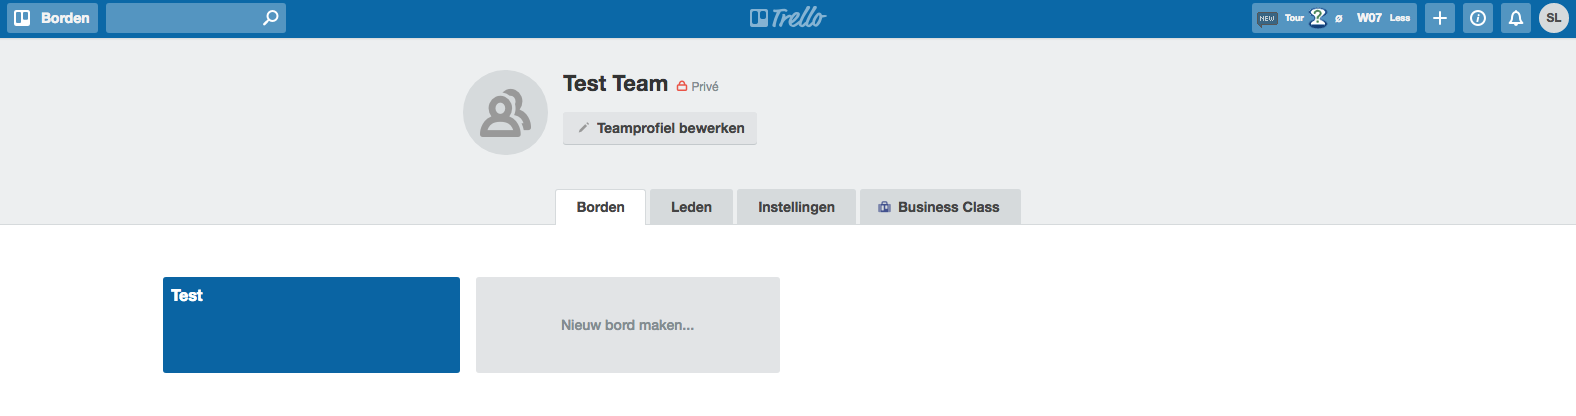
\includegraphics[width=\textwidth]{./afbeeldingen/overzicht_team.png}
	\caption{Overzichtscherm van een team}
	\label{fig:overzicht_team}	
\end{figure} 

\section{Team aanmaken}

Om een nieuw team aan te maken heb je de keuze uit deze 2 manieren:
\begin{itemize}
	\item Vanuit hoofdscherm Trello
	\begin{enumerate}[nolistsep]
		\item Scroll helemaal naar onder;
		\item Kies de optie ``Maak een nieuw team aan ...''.
	\end{enumerate}
\pagebreak
	\item Vanuit het detailscherm van hetTrellobord (van dat team)
	\begin{enumerate}[nolistsep]
		\item Klik op de teamnaam;
		\item Kies ``Wijzig team ...'' (Enkel als er al een team gekozen is anders vervalt deze stap);
		\item Kies ``Team cre\"eren.
	\end{enumerate}
\end{itemize}

\noindent
\\Vul daarna de gegevens aan \korteverwijzing[fig:aanmaken_team] en bevestig deze om het team effectief aan te maken. Nadien wordt het overzichtscherm van het team getoond \korteverwijzing[fig:overzicht_team]. Het is ook mogelijk om hier een nieuw bord aan te maken voor dat team.

\begin{figure}[H]
	\centering
	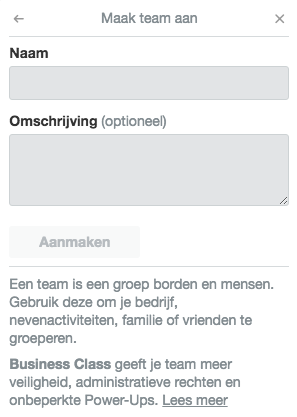
\includegraphics[scale=0.6]{./afbeeldingen/aanmaken_team.png}
	\caption{Aanmaken van een team}
	\label{fig:aanmaken_team}	
\end{figure} 

\section{Team wijzigen}

Om een team te wijzigen volstaat het om zijn overzichtspagina te openen van waaruit je toegang hebt tot volgende mogelijkheden:
\begin{itemize}
	\item Teamprofiel aanpassen;
	\item Leden toevoegen / verwijderen;
	\item Rechten van leden aanpassen;
	\item Teaminstellingen aanpassen.
\end{itemize}

\section{Team verwijderen}

Om een team te kunnen verwijderen voer je volgende stappen uit:
\begin{enumerate}[nolistsep]
	\item Open de teampagina;
	\item Selecteer ``instellingen'';
	\item Kies de optie ``Dit team verwijderen?'' onderaan de pagina;
	\item Bevestig het verwijderen.
\end{enumerate}

\noindent
\\Als je het team verwijdert van het huidige bord zal dit de waarde ``Persoonlijk'' voor zijn team krijgen.